\documentclass{beamer}
\usetheme{Frankfurt}
\setbeamertemplate{footline}[frame number]
\setbeamercovered{transparent}
\usepackage{graphicx}
\usepackage{animate}
\graphicspath{{../images/}{../videos/}{../videos/test/}}
\usepackage{tikz}
\usepackage{media9}
\addmediapath{../videos/}


\title{SPH simulations for space defense}
\author{Maximilian Rutz}

\begin{document}
\begin{frame}[plain]
    \maketitle
\end{frame}
\begin{frame}[plain]{Roadmap}
\tableofcontents
\end{frame}
\section{Dart and Hera Missions}
\begin{frame}
	\begin{tikzpicture}[remember picture,overlay]
	\node[at=(current page.center)] {
		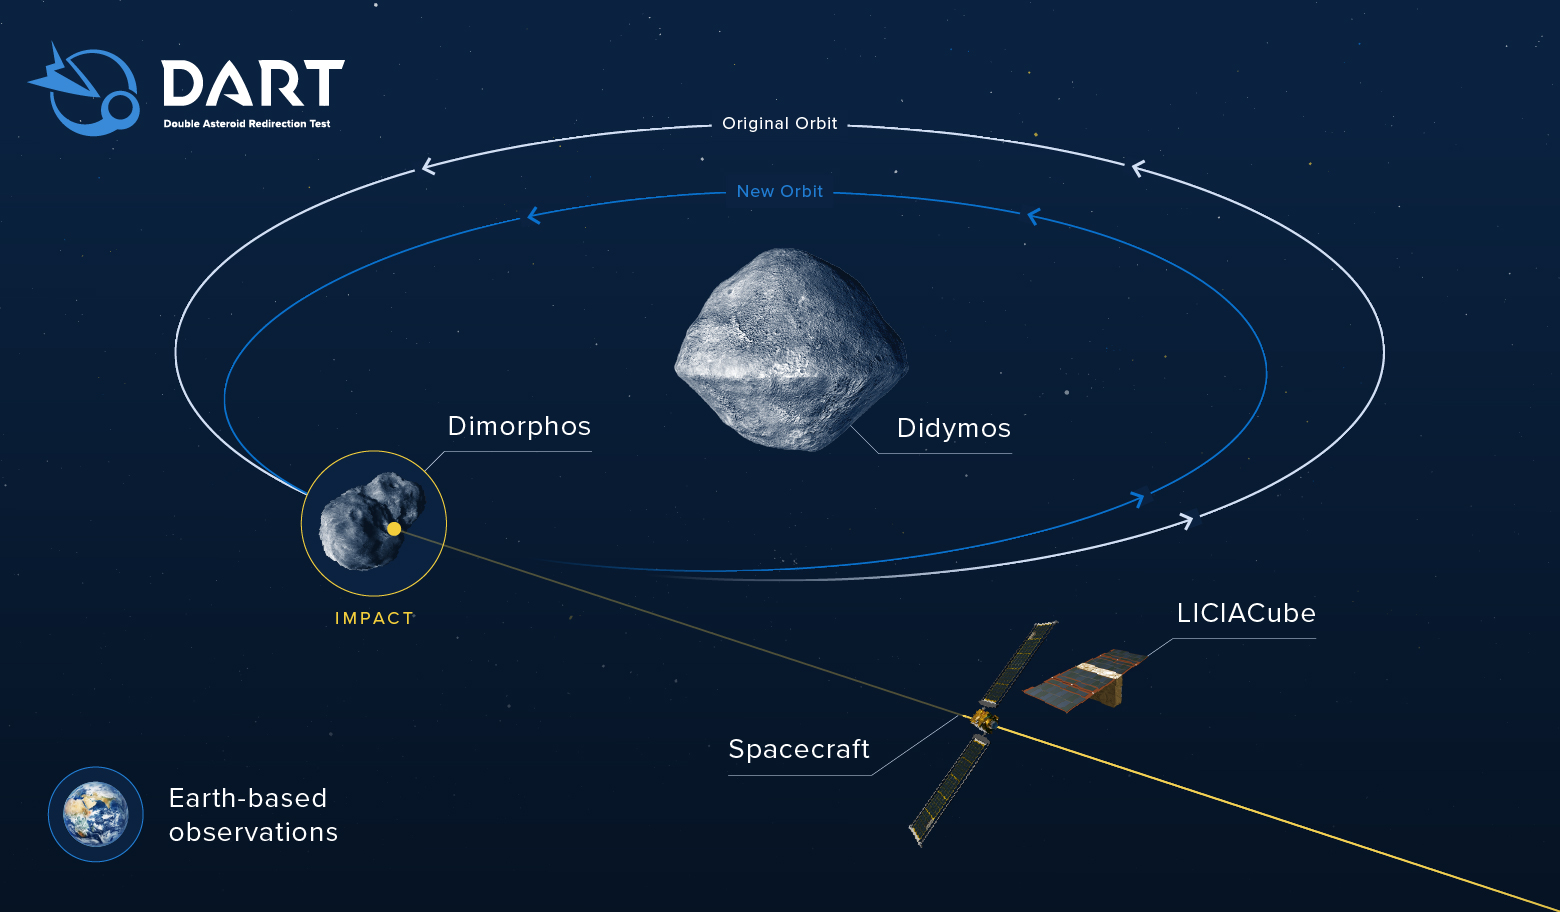
\includegraphics[keepaspectratio,
		width=\paperwidth,
		height=\paperheight]{dart_mission.jpg}};
	\end{tikzpicture}
\end{frame}

\begin{frame}{Target}
	Didymos 
\end{frame}
\begin{frame}{Impactor}
	DART 
\end{frame}
\section{SPH setup}
\begin{frame}{SPH method}
	Smoothed particle hydrodynamics
\end{frame}
\begin{frame}{Miluphcuda}
	Smoothed particle hydrodynamics
\end{frame}
\begin{frame}{Miluphcuda setup}
	\begin{itemize}
		\item xˆ3 Kernel function \pause
		\item artifical viscosity \pause
		\item Runge Kutta Fourth order \pause
		\item no self gravity \pause
		\item p-$\alpha$ porosity - micro vs macroporosity\pause
	\end{itemize}
\end{frame}
\begin{frame}{Initial conditions setup}
	\begin{itemize}
		\item xˆ3 Kernel function \pause
		\item artifical viscosity \pause
		\item Runge Kutta Fourth order \pause
		\item no self gravity \pause
		\item p-$\alpha$ porosity \pause
	\end{itemize}
\end{frame}
\begin{frame}{smoothing length}
	- how can resolution be locally increased with SPH method (different radii and sml)
	- limit of sml -> 0 is normal hydrodynamics??
\end{frame}
\section{SPH results}
\begin{frame}{Beta factor}
\end{frame}
\begin{frame}{Target porosity and strength}
	\animategraphics[loop,controls,width=0.8\linewidth]{100}{binac}{0000}{0300}
	exemplary video
\end{frame}
\begin{frame}{Comparision with grid codes}
	Raducan
\end{frame}

\begin{frame}{Impact angle}
	Not seen in 2d grid codes Raducan
\end{frame}
\begin{frame}{Conclusion}
\end{frame}
\begin{frame}[plain]{The Chelyabinsk meteor 2013}
	\includemedia[
	activate=onclick,
	width=0.75\textwidth
	]{}{chelyabinsk.swf}
\end{frame}

\end{document}